\documentclass{beamer}
\usetheme{metropolis}           % Use metropolis theme
\metroset{numbering=fraction}
\usepackage[T2A]{fontenc}
\usepackage[utf8]{inputenc}
\usepackage[english,russian]{babel}
\usepackage{minted}
\usepackage{soul}

\title{Декларативное программирование}
\subtitle{Семинар №9, группа 22215}
\author{Завьялов А.А.}
\date{31 октября 2022 г.}
\institute{Кафедра систем информатики ФИТ НГУ}
\begin{document}
  \maketitle
  \begin{frame}[fragile]{Классы типов}
      \begin{itemize}
          \item Один из механизмов \textit{обобщенного} программирования в Haskell
          \item Описывают множество типов с одним набором операций 
      \end{itemize}
      \begin{minted}{haskell}
    class  (Eq a) => Ord a  where
        compare              :: a -> a -> Ordering
        (<), (<=), (>), (>=) :: a -> a -> Bool
        max, min             :: a -> a -> a
        {-# MINIMAL compare | (<=) #-}
        
    data Bin = Zero | One deriving (Eq)
    instance Ord Bin where
        Zero <= One = TRUE
        x <= y = x == y
     \end{minted}
  \end{frame}
  \begin{frame}{Стандартные классы типов}
      \begin{itemize}
          \item \texttt{Eq} -- отношение эквивалентности
          \item \texttt{Ord} -- отношение \textit{полного} порядка
          \item \texttt{Show} -- перевод в строку
          \item \texttt{Read} -- чтение из строки
          \item \texttt{Enum} -- \href{https://en.wikipedia.org/wiki/Computably_enumerable_set}{перечислимое  множество}
          \item \texttt{Bounded} -- \href{https://en.wikipedia.org/wiki/Infimum_and_supremum}{множество с точной верхней и нижней границами}
      \end{itemize}
      \begin{itemize}
          \item \texttt{Num} -- арифметические операции
            \begin{itemize}
                \item \texttt{Integral} -- целые числа
                \item \texttt{Real} -- вещественные числа
            \end{itemize}
      \end{itemize}
  \end{frame}
  \begin{frame}{Иерархия некоторых стандартных классов типов}
      \begin{figure}
          \centering
          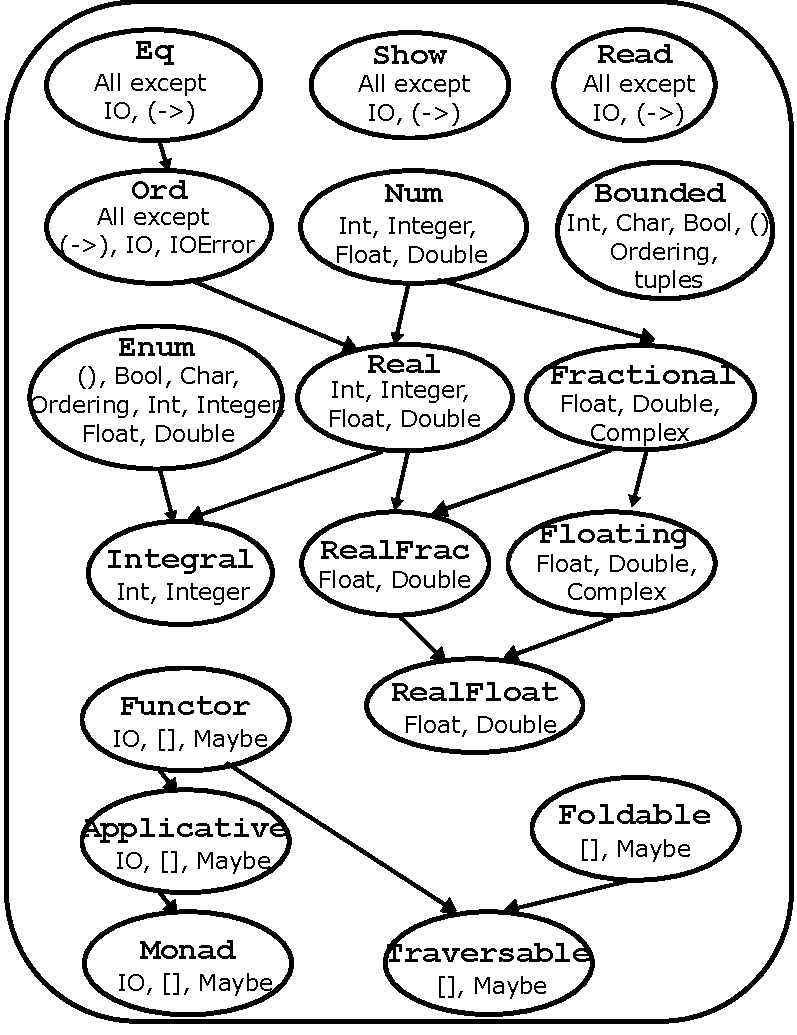
\includegraphics[scale=0.45]{media/base-classes.pdf}
      \end{figure}
  \end{frame}
  \section{Полугруппы, моноиды}
  \begin{frame}[fragile]{Класс типов \texttt{Semigroup}}
      \begin{itemize}
          \item Полугруппа --- множество с заданной на нём \textbf{ассоциативной} операцией $(S,\cdot)$.
      \end{itemize}
      \begin{minted}{haskell}
        class Semigroup a where
            (<>) :: a -> a -> a
      \end{minted}
      
      \begin{block}{Примеры}
        \begin{itemize}
            \item Списки и операция конкатенации \texttt{(++)}
            \item Упорядоченное множество с операцией минимума (максимума) из двух элементов
        \end{itemize}
      \end{block}
      \begin{block}{Свойство полугруппы (semigroup law)}
        \begin{itemize}
            \item \mintinline{haskell}{x <> (y <> z) = (x <> y) <> z} --- ассоциативность
        \end{itemize}
      \end{block}
  \end{frame}
  \begin{frame}[fragile]{Класс типов \texttt{Monoid}}
      \begin{itemize}
          \item Моноид --- полугруппа с нейтральным элементом (''единицей'').
      \end{itemize}
      \begin{minted}{haskell}
        class Semigroup a => Monoid a where
            mempty  :: a
            mappend :: a -> a -> a
            mappend = (<>)
            mconcat :: [a] -> a
      \end{minted}
      \begin{block}{Свойства моноида (monoid laws)}
        \begin{itemize}
            \item \mintinline{haskell}{x `mappend` mempty = x} 
            \item \mintinline{haskell}{mempty `mappend` x = x}
            \item \mintinline{haskell}{x <> (y <> z) = (x <> y) <> z} --- ассоциативность
        \end{itemize}
      \end{block}
  \end{frame}
  \begin{frame}{Примеры моноидов}
        \begin{itemize}
            \item Целые числа, 0 и операция \alert{сложения}
            \item Целые числа, 1 и операция \alert{умножения}
            \item Булевы значения, False и логическое ''или''
            \item Булевы значения, True и логическое ''и''
            \item Списки, пустой список и операция конкатенации
            \item Ограниченное снизу (сверху) множество, операция минимума (максимума) из двух и нижняя (верхняя) грань
        \end{itemize}
  \end{frame}
  \begin{frame}[fragile]{Практическое применение моноидов}
      \begin{block}{Ассоциативность решает}
        \begin{minted}{haskell}
  foldl mappend mempty col = foldr mappend mempty col
  fold mappend mempty [] = mempty
  mconcat = foldr mappend mempty
        \end{minted}
      \end{block}
      \begin{itemize}
          \item Ассоциативность $\equiv$ порядок вычислений не важен
          \item Свёртка над списком моноидов -- дополнительная гарантия, что вы получите нужный результат
            \begin{itemize}
                \item при условии, что выполнены \alert{законы моноидов}
            \end{itemize}
      \end{itemize}
  \end{frame}
  \section{Функторы, в том числе, аппликативные}
  \begin{frame}[fragile]{Тип данных \texttt{Maybe}}
    \texttt{Maybe} моделирует ситуацию, когда значение может отсутствовать:
    \begin{minted}{haskell}
  data Maybe a  =  Nothing | Just a
    \end{minted}
    \begin{block}{Возможные подходы к обработке отсутствующих значений}
        \begin{itemize}
            \item Элемента нет -- бросаем исключение, затем обрабатываем (C\#, Java)
            \item Элемента нет -- возвращаем \texttt{null} (Алгол, C, C++, C\#, Java, \textit{etc})
            \item Элемент есть -- возвращаем \mintinline{haskell}{Just elem}, элемента нет -- возвращаем \mintinline{haskell}{Nothing} (Haskell, Rust, Swift, Kotlin, \textit{большинство современных языков})
        \end{itemize}
    \end{block}
  \end{frame}
  \begin{frame}[fragile]{Работа с \texttt{Maybe}}
      Использование \texttt{Maybe} делит иерархию типов программы на обычные (\texttt{a, [a], Int, ...}) и типы, значение которых может отсутствовать (\texttt{Maybe a, Maybe [a], Maybe Int, ...})
      
      \begin{block}{Очевидный подход к использованию \texttt{Maybe}}
\begin{minted}{haskell}
showFromMaybe :: Show a => Maybe a -> String
showFromMaybe Nothing = ""
showFromMaybe (Just x) = show x
\end{minted}
      \end{block}
  Круто, модно, но есть одна проблема... 
  \end{frame}
  \begin{frame}[fragile]{Работа с \texttt{Maybe}}
      Есть \mintinline{haskell}{Just 42}, нужно прибавить к значению внутри единицу.
      \begin{block}{Не вопрос!}
  \begin{minted}{haskell}
    addOneToMaybe :: Maybe Int -> Maybe Int
    addOneToMaybe Nothing = Nothing
    addOneToMaybe (Just x) = Just (succ x)
\end{minted}
      \end{block}
      \begin{block}{Но...}
        \begin{itemize}
            \item Неужели всегда нужно писать так много кода?
            \item Неужели нужно всё выносить в отдельные функции?
            \item Как такие функции комбинировать между собой?
        \end{itemize}
      \end{block}
  \end{frame}
  \begin{frame}[fragile]{Functors to the rescue!}
      \begin{minted}{haskell}
    class Functor f where
        fmap :: (a -> b) -> f a -> f b
        
    >fmap succ (Just 42)
    Just 43
    >fmap succ Nothing
      \end{minted}
      \begin{itemize}
          \item \alert{обратите внимание}: \texttt{f} -- тип с параметром
          \item \texttt{fmap} выполняет операцию \texttt{a -> b} внутри типа \texttt{f}, и переводит значение типа \texttt{f a} в значение типа \texttt{f b}
          \item можно считать, что мы преобразовали функцию \texttt{\textbf{a -> b}} в функцию \texttt{\textbf{f a -> f b}} (''подняли'' (англ. -- lift) вычисление в функтор)
      \end{itemize}
  \end{frame}
  \begin{frame}[fragile]{Функторы}
    \begin{block}{Законы функторов}
      \begin{itemize}
          \item \mintinline{haskell}{fmap id == id} -- закон тожедственности (Identity)
          \item \mintinline{haskell}{fmap (f . g) == fmap f . fmap g} -- закон композиции (Composition)
      \end{itemize}
      \end{block}
      \begin{block}{Использование функторов}
        \begin{minted}{haskell}
    >fmap (+1) [1,2,3]
    [2,3,4]
    >(+1) <$> [1,2,3]
    [2,3,4]
    > (+1) $ 2
    3
        \end{minted}
      \end{block}
  \end{frame}
  \begin{frame}{Типы, реализующие класс \texttt{Functor}}
      \begin{itemize}
          \item \texttt{Maybe}
          \item \mintinline{haskell}{[]}
          \item \texttt{(,)} \alert{(!)}
          \item И многие другие...
      \end{itemize}
  \end{frame}
  \begin{frame}[fragile]{Где функторы бессильны...}
     \begin{minted}{haskell}
    -- Унарная операция (a -> b), всё ok
    (+1) <$> Just 1
    
    -- Бинарная операция, ???
    (+) <$> Just 1 ??? Just 2
    
    fmap (+) :: (Num a, Functor f) => f (a -> a)
    -- С значениями вида f (a -> b)
    -- уже ничего не можем сделать...
     \end{minted}
  \end{frame}
  \begin{frame}[fragile]{...найдется дело для аппликативных функторов!}
      \begin{minted}{haskell}
    class Functor f => Applicative f where
        pure :: a -> f a
        (<*>) :: f (a -> b) -> f a -> f b
        
    
    -- Бинарная операция? Легко!
    (+) <$> Just 1 <*> Just 2
    -- Just 3
      \end{minted}
  \end{frame}
  \begin{frame}{Типы, реализующие класс \texttt{Applicative}}
      \begin{itemize}
          \item \texttt{Maybe}
          \item \mintinline{haskell}{[]}
          \item \st{\texttt{(,)}} \alert{Почему?}
          \item И многие другие...
      \end{itemize}
  \end{frame}
  \begin{frame}{Список как аппликативный функтор}
      Моделирует недетерминированные вычисления:
      \begin{figure}
          \centering
          
\includegraphics[width=0.95\textwidth]{media/dr-strange.jpg}
      \end{figure}
  \end{frame}
  \section{QuickCheck и проверка свойств}
  \section{Q\&A}
\end{document}